\documentclass{article}
\usepackage[utf8]{inputenc}
\usepackage[icelandic]{babel}
\usepackage[T1]{fontenc}
\usepackage{graphicx}
\usepackage{mathtools}
\usepackage{amsmath}
\usepackage{amssymb}
\usepackage{minted}


\graphicspath{ {./} }
\title{Vikublað 10 - tölvunarfræði 2}
\author{ttb3@hi.is}
\date{\today}


\begin{document}
\maketitle


\section*{4.1.14}
BFS notar \emph{queue} til að geyma upplýsingar um hnúta sem búið er að skoða.
Þetta gerir BFS kleift að finna stysta veg á milli tveggja hnúta.
Ef við myndum nota \emph{stack} myndi það hafa áhrif á leitina á þann hátt að öll önnur hliðin væri farin áður en byrjað væri að skoða hina.
Frekar illa orðað en sjá teikningar,
\begin{center}
    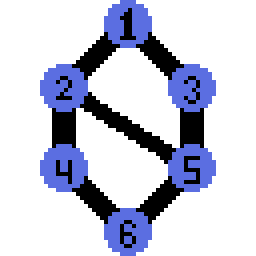
\includegraphics{graph.png}
\end{center}
Ef við byrjum með þetta tré og förum snöggt í gegnum það hvernig leitað væri í því með BFS þar sem er notað \emph{queue}.
Q táknar queue, P táknar print. Hver lína felur í sér að prenta næsta hnút í röðinni og setja tengda hnúta í röðina. Við byrjum á 1.\\

\begin{tabular}{|l|l|}
    \hline
    P&Q\\
    \hline
                &1\\
                \hline
    1           &2,3\\
    \hline
    1,2         &3,4,5\\
    \hline
    1,2,3       &4,5\\
    \hline
    1,2,3,4     &5,6\\
    \hline
    1,2,3,4,5   &6\\
    \hline
    1,2,3,4,5,6 &\\
    \hline
\end{tabular}

Sjáið núna muninn ef við notum \emph{stack} en ekki \emph{queue}:
\begin{align*}
    P:&[] & S:[]&\\ 
    P:&[] & S:[]&\\ 
    P:&[] & S:[]&\\ 
    P:&[] & S:[]&\\ 
    P:&[] & S:[]&\\ 
    P:&[] & S:[]&\\ 
    P:&[] & S:[]& 
\end{align*}

\end{document}